In this section, we discuss the performance of an SPH simulation code
with self-gravity implemented using FDPS.  Some results in this
scetion have been published in \citet{2015FDPS}.  The test problem
used is the simulation of GI. The GI
hypothesis \citep{1975Icar...24..504H, 1976LPI.....7..120C} is one of
the most popular scenarios for the formation of the Moon. The
hypothesis is as follows. About 5 billion years ago, a Mars-sized
object (hereafter, the impactor) collided with the proto-Earth
(hereafter, the target). A large amount of debris was scattered, which
first formed the debris disk and eventually the Moon. Many researchers
have performed simulations of GI, using the SPH method
\citep{1986Icar...66..515B, 2013Icar..222..200C, 2014NatGe...7..564A}.

For the gravity, we used monopole-only kernel with $\theta=0.5$. We
adopt the standard SPH scheme
\citep{1992ARA&A..30..543M, 2009NewAR..53...78R, 2010ARA&A..48..391S}
for the hydro part. Artificial viscosity is used to handle shocks
\citep{1997JCoPh.136..298M}, and 
the standard Balsara switch is used to reduce the shear viscosity
\citep{1995JCoPh.121..357B}. A kernel function we used is the Wendland $C^6$ and the cutoff radius
is 4.2 times larger than the local mean inter-particle distance. In
other words, each particle interact with about 300 particles. This
neighbor number is the appropriate for this kernel to avoid the
pairing instability \citep{2012MNRAS.425.1068D}.


%In all simulations, we set the cutoff radius to be 4.2 times larger
%than the local mean inter-particle distance. In other words, each
%particle interact with about 300 particles.

%In all GI simulations, we make three instances of
%class \texttt{TreeForForce}. One is for evaluating the density and the
%smoothing length of the kernel function for i-th particle. The second
%tree is for solving the Euler equation. In other words, we evaluate
%pressure gradient, the artificial viscosity and the Balsara switch
%with this tree.  The other tree is for gravity force.

Assuming that the target and impactor consist of granite, we adopt
equation of state of granite \citep{1986Icar...66..515B} for the
particles. For the initial condition, we assume the parabolic orbit
with the initial angular momentum 1.21 times of the current Earth-Moon
system.

%The initial conditions, such as the orbital parameters of
%the two objects, are the same as those in \citet{1986Icar...66..515B}.

%In this paper, we report the weak scaling performance with about 250k
%particles per cores. For the largest calculation, we used $1.0$
%billion particles and $4096$ nodes.

\begin{figure}
  \begin{center}
    \includegraphics[width=8cm]{figure/GI.eps}
  \end{center}
  \caption{Temperature maps of the target and impactor in the run with
  $9.9$ million particles at four different epochs. }
  \label{fig:evolutionGI}
\end{figure}

Figure~\ref{fig:evolutionGI} shows the time evolution of the target
and impactor for a run with 9.9 million particles. We can see that the
shocks are formed just after the moment of impact in both the target
and impactor ($t=2050$ sec). The shock propagates in the target, while
the impactor is completely disrupted ($t=2847$ sec) and debris are
ejected. A part of the debris falls back to the target, while the rest
will eventually form the disk and the Moon. So far, the resolution
used in the published papers have been much lower. We plan to use this
code to improve the accuracy of the GI simulations.

Figure~\ref{fig:gi_weak} and \ref{fig:gi_strong} show the measured
weak and strong scaling performance. For the weak-scaling measurement,
we fixed the number of particles per core to 20,000 and measured the
performance for the number of cores in the range of 256 to 131,072 on
the K computer. On the other hand, for the strong-scaling measurement,
we fixed the total number of particles to $39$ million and measured
the performance for the number of cores in the range of 512 to 16,384
on K computer. We can see that the performance is good even for very
large number of cores. The efficiency is about 40\% of the theoretical
peak performance. The hydro part consumes more time than the gravity
part does, mainly because the particle-particle interaction is more
complicated.

%Figure~\ref{fig:gi_strong} shows the measured strong-scaling
%performance. We fixed the total number of particles to $39$ million
%and measured the performance for number of cores in the range of 512
%to 16384 on K compute.

\begin{figure}
  \begin{center}
    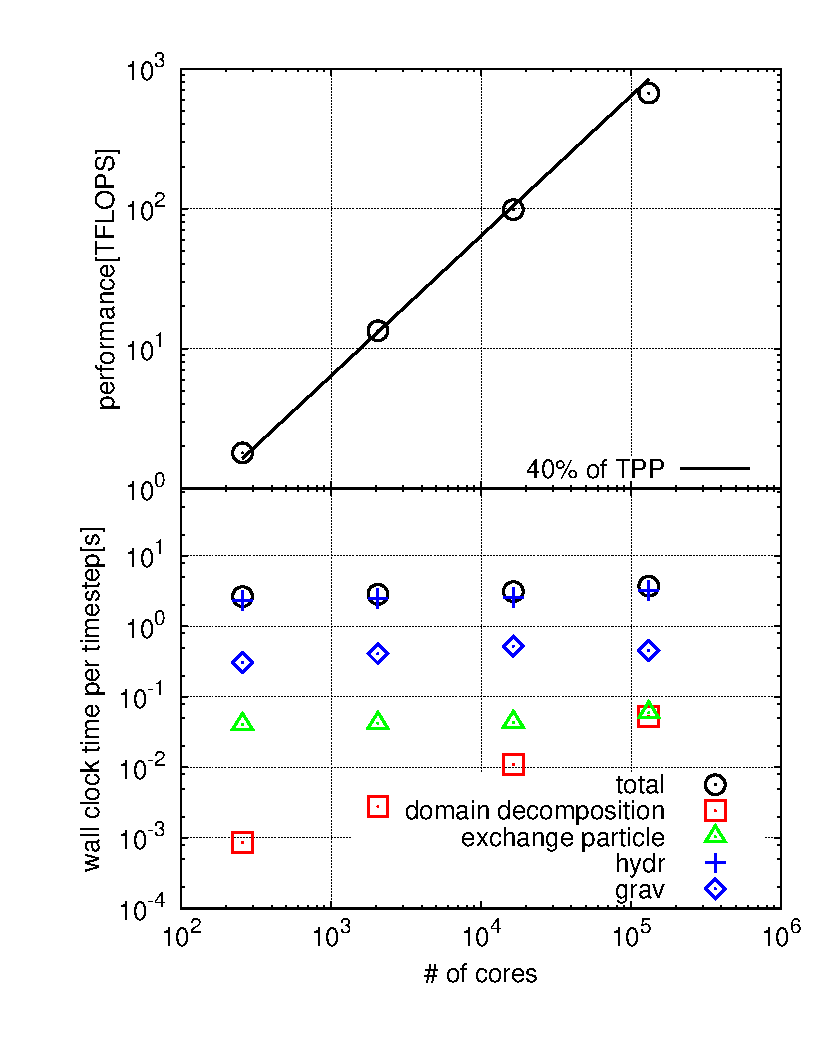
\includegraphics[width=8cm]{figure/gi_weak.eps}
  \end{center}
  \caption{

    Weak-scaling performance of the SPH code. The speed of the
    floating-point operation (top) and wallclock time per one timestep
    (bottom) are plotted as functions of the number of cores. In the
    top panel, the solid line indicates 40\% of the theoretical peak
    performance of K computer. In the bottom panel, time spent for the
    hydrodynamics calculation (cross), the gravity calculation
    (diamond), the domain decomposition (square) the exchange
    particles (triangle) are also shown.

}
  \label{fig:gi_weak}
\end{figure}

\begin{figure}
  \begin{center}
    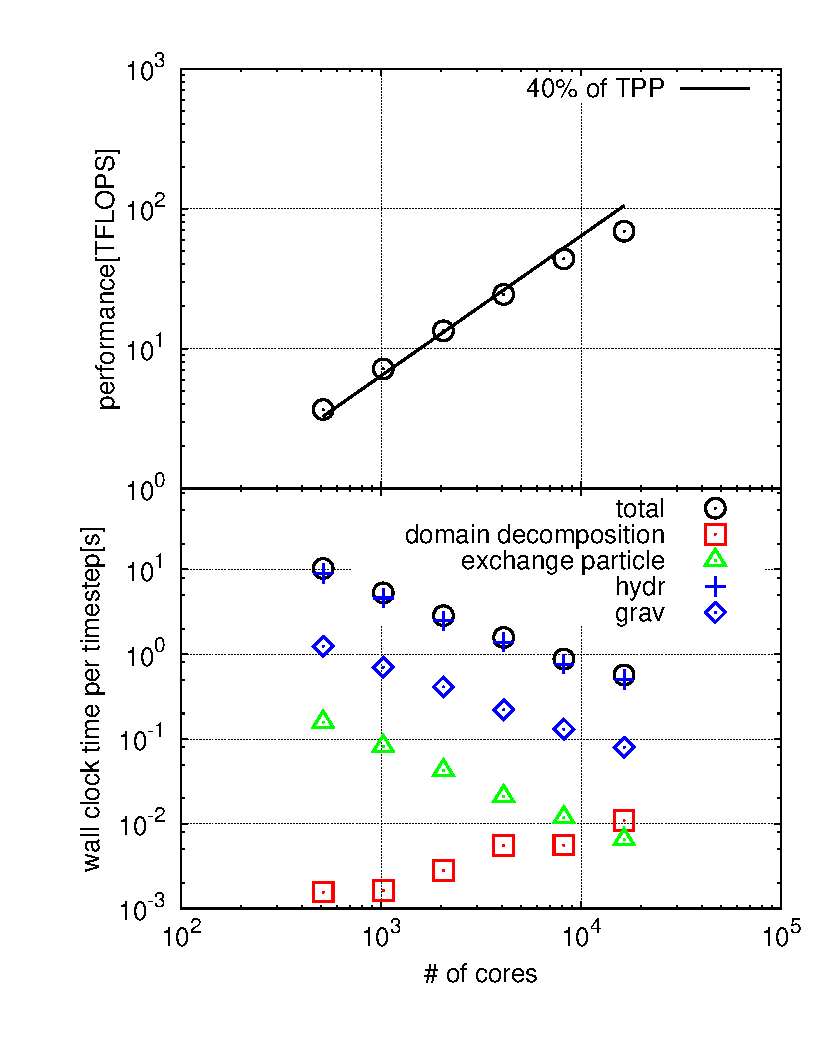
\includegraphics[width=8cm]{figure/gi_strong.eps}
  \end{center}
  \caption{

The same as figure \ref{fig:gi_weak} but for the strong-scaling
performance for $39$ million particles.

}
  \label{fig:gi_strong}
\end{figure}


%The largest number of particles used for GI simulations so far
%reported is 100 million \cite{2014LPI....45.2703T}. Unfortunately,
%performance numbers are not given. After we replace the interaction
%kernels with SIMD-optimized ones for hydrodynamics part, we believe we
%can achieve the performance not so much lower than that we achieved
%for pure gravity calculation.

% LocalWords:  SPH FDPS impactor proto Balsara rr rrr Grav Wendland SIMD

% LocalWords:  builtin Wallclock timestep wallclock monopole
